\documentclass[10pt, a4paper, twoside]{article}


% Set up the standard margins for the document
% 42.2 left & 15.5 right is same as Forsling, Neymark
% 21.3 top  & 20 bottom is same as Olofsson
\usepackage[left=15.5mm, right=15.5mm, top=21.3mm, bottom=20mm]{geometry}

% Input file character encoding (kinda useless if we don't
% use åäö and stuff, but it doesn't hurt to have it)
\usepackage[utf8]{inputenc}

% Block Comments
\usepackage{comment}

% No indentation in new paragraph
\usepackage{parskip}

% To include graphics
\usepackage{graphicx}

% More mathematical symbols and fonts
\usepackage{amsmath}
\usepackage{amsfonts}
\usepackage{amssymb}

% Simple list
\usepackage[ampersand]{easylist}
\ListProperties(Hide=100, Hang=true, Progressive=5ex, Style*=$\bullet$ ,
Style2*=-- ,Style3*=$\circ$ ,Style4*=\tiny$\blacksquare$ )


% Clickable internal links
\usepackage{hyperref}
\usepackage[all]{hypcap} % without this the link takes you to the caption, not the top of the image
\hypersetup{ % Settings for links in documnet
	setpagesize = false, % Don't allow hyperref to change page size. Tips från Micke Olofsson
	colorlinks = true,   % No boxes around links
	linkcolor = black,citecolor = black,filecolor = black,urlcolor = black, % don't color links
}

% To include to first page pdf file
\usepackage{pdfpages}

% Add section number to equation and figure number (ex: 5.11 instead of simply 11)
\numberwithin{equation}{subsection}
\numberwithin{figure}{section}
\numberwithin{table}{section}

% Show program code listings in document
\usepackage{listings}

%
% Header stuff
%
\usepackage{fancyhdr}
\setlength{\headheight}{15pt}

\fancyhf{}
\fancyhead[LE, RO]{\thepage}
\fancyhead[RE]{TSBB15 2013: Project Report}
\fancyhead[LO]{Object Tracking in Image Sequences}

\fancypagestyle{plain}{ %
\fancyhf{} % remove everything
\renewcommand{\headrulewidth}{0pt} % remove lines as well
\renewcommand{\footrulewidth}{0pt}}
%
% End header stuff
%




\begin{document}

% First page

\includepdf{Cover/cover.pdf}


% Project identity page
\newpage
\pagestyle{fancy}
\pagenumbering{roman}
\setcounter{page}{2} % sets the current page number to 2 

\begin{center}
    \vspace*{4\baselineskip}

	\textbf{\huge PROJECT IDENTITY} \\
	\vspace*{0.5\baselineskip}
	Computer Vision, VT 2013, group 2 \\
	Department of Electrical Engineering (ISY), Link\"{o}ping University
	
	\vspace*{2\baselineskip}
	\textbf{\LARGE Participants}


	{\footnotesize 
	\begin{tabular}{|p{2.7cm}|p{5cm}|p{2cm}|p{3.4cm}|}
		\hline
			\textbf{Name} & \textbf{Responsibilities} & \textbf{Phone} & \textbf{E-mail} \\
		\hline
		Gustav Häger & Background modelling &  & gusha124@student.liu.se \\
		\hline
		Alexander Sjöholm & Kalman prediction, \newline Evaluation of results &  & alesj050@student.liu.se \\
		\hline
		Martin Svensson & Foreground segmentation & 070--289\,01\,49 & marsv106@student.liu.se \\
		\hline
		Mattias Tiger & Object identification &  & matti166@student.liu.se \\
		\hline
	\end{tabular}
	}

{\footnotesize 
\textbf{E-mail list to the group}: marsv106@student.liu.se \\
\vspace{1\baselineskip}

%\textbf{Customer}: Some Guy, Link\"{o}ping University \\
%\textbf{Customer contact}: 333--33\,33\,33, 070--333\,33\,33, Fax: 013--33\,33\,33, some_guy@some_domain.se \\
\textbf{Project supervisor}: Fahad Khan, Link\"{o}ping University, fahad.khan@liu.se \\
\textbf{Course leader}: Per-Erik Forssén, 013--28\,56\,54, per-erik.forssen@liu.se \\
}

\end{center}



% table of contents
\newpage
\tableofcontents
\listoffigures
%\listoftables

% list of figures
%\newpage
%\listoffigures


% Document history page
\newpage
\vspace*{5\baselineskip}

\begin{center}
\textbf{\LARGE Document history}

{ \footnotesize 
\begin{tabular}{|p{1cm}|p{2.0cm}|p{5cm}|p{1.5cm}|p{2cm}|}
	\hline
	\textbf{Version} & \textbf{Date} & \textbf{Changes} & \textbf{Sign} & \textbf{Reviewed} \\
	
	\hline
	0.1 & 2013--03--19 & Initial draft & MS & GH, MT\\
	
	\hline
	0.2 & 2013--03--28 & Second draft & MS & GH, MT\\
	
	\hline
	0.3 & 2013--04--01 & Third draft & AS & MT, MS\\
	
	\hline
	1.0 & 2013--04--03 & Final version & AS & MT, MS, GH\\
	
	\hline
	 &  &  &  &  \\
	
	\hline
\end{tabular}
}
\end{center}


% Blank page
%\newpage
%\thispagestyle{empty}
%\mbox{}



%
% Content start
%
\newpage
\pagenumbering{arabic}

\newpage
\section{Introduction}
This document is the final documentation of a mini-project performed as a part of the course Computer Vision (TSBB15) at Linköping university. The purpose of the project is to implement a tracker capable of handling occlusion, shadows and changes in the background. Object tracking is, in computer vision, defined as the process where moving objects are located in a image sequence. The project goal was to create a real-time tracker to work on e.g. a surveillance camera and track the people and objects in its view. The application was implemented in C++ using the OpenCV API.

The purpose of this document is to provide a thorough description of how the application was created and the problems encountered during the implementation work.


\section{System description}
The system implementation is divided into four main modules, Feature extraction, Pose estimation, Non-linear optimization and 3D visualization.

\begin{figure}[htb]
	\centering
	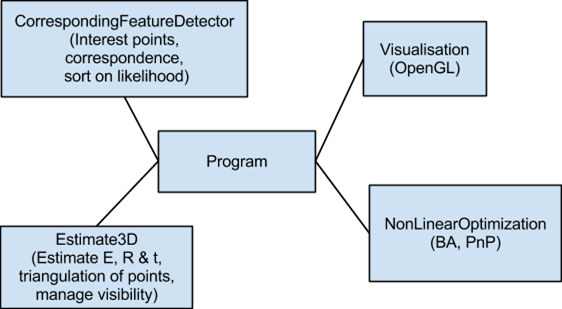
\includegraphics[width=110mm]{images/system_modules.png}
	\caption{\textit{Modules of the system}}
	\label{fig:block_overview2_fig}  %Skapar referens till figuren
\end{figure}

First feature extraction using Harris is performed as a preprocessing step on all images. These are used to calculate pairwise image point correspondences using SIFT.

Then an iterative process is performed cycling though all camera-pairs, each consisting of two parts. The first part contains an initial camera pose estimation, of the new camera, using the essential matrix estimated from F using the Gold standard algorithm. The camera pose is then improved using PnP on all previously known 3D-points and over all cameras. An initial 3D-point triangulation is then calculated.
The second part is a bundle adjustment over all current 3D points and cameras by the means of a non-linear optimization.

When all camera poses and estimated 3D-points have been iteratively added and optimized the result is rendered using OpenGL.

\begin{figure}[htb]
	\centering
	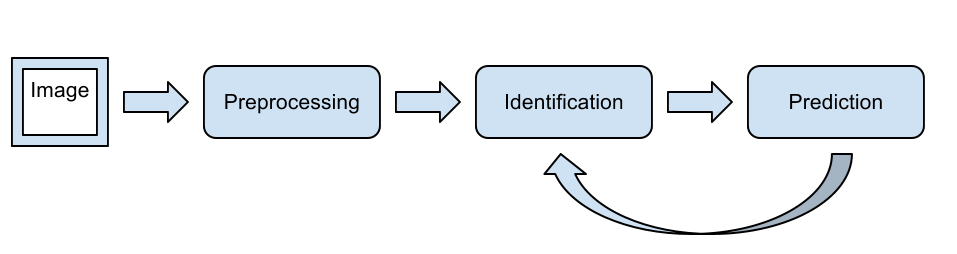
\includegraphics[width=120mm]{images/data_flow.png}
	\caption{\textit{Data flow between modules.}}
	\label{fig:block_overview_fig}  %Skapar referens till figuren
\end{figure}


\newpage
\subsection{Main Program}
The main program is composed of two parts. The first one is initiation part, where the modules are declared, parameters specified, and movie clip loaded. The second one is the main loop, where the actual program is executed.


\subsubsection{Main loop}
When the program is started and the initiation is done the program is set to run until the end of the specified movie sequence. For each frame in the sequence, the Background model is updated and a probability map matrix containing information about what pixels are part of the background is created. After the probability map has been created, the foreground processing module is called upon to perform some noise removal and to detect all the interesting regions in the probability map (the regions that are likely to be part of the foreground). 

Once all the interesting regions are labeled, the identification module takes all the created objects in the current frame and associates them with the proper ID. This is done by comparison with the objects in the previous frame.

To help in the labeling process we use a Kalman predictor, that predicts the position of the each object in the next frame. The Prediction module is called upon after the identification is done.

Once all the processing in the module is finished the objects in the current frame are drawn in the current frame as bounding boxes with velocity vectors, position in pixel coordinates and ID numbers.


See code in appendix \ref*{sec:Main_code}. %referens till kod, ger klickbar l�nk.

\begin{figure}[htb]
	\centering
	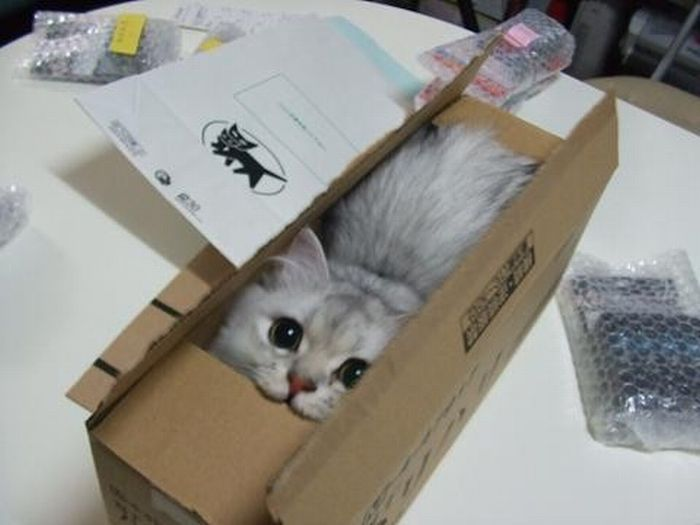
\includegraphics[width=\linewidth]{images/acatisfinetoo}
	\caption{\textit{Some flowchart of main program.}}
	\label{fig:MainProgram_fig} %Skapar referens till figuren
\end{figure}



\newpage
\subsection{Data structures}
In order to keep a good structure on the program and a logical separation of functionalities, several data structures have been created.

\begin{figure}[htb]
	\centering
	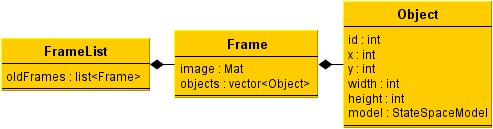
\includegraphics[width=150mm]{images/data_structures_uml.png}
	\caption{\textit{UML diagram of the main data structures. A video is represented by a FrameList, containing each Frame of the video. Each such Frame contains the detected objects in that image and each object contains spatial information, a unique id and a StateSpaceModel used for the Kalman filter prediction}}
	\label{fig:UML_fig} %Skapar referens till figuren
\end{figure}

%\subsubsection{ProbabilityMap}
%DErpa derpa derpa derpa. DErpa derpa derpa derpa.DErpa derpa derpa derpa.DErpa derpa derpa derpa.DErpa derpa derpa derpa.DErpa derpa derpa derpa.DErpa derpa derpa derpa.
%DErpa derpa derpa derpa.DErpa derpa derpa derpa.DErpa derpa derpa derpa.DErpa derpa derpa derpa.DErpa derpa derpa derpa.DErpa derpa derpa derpa.DErpa derpa derpa derpa.
%DErpa derpa derpa derpa. See code in appendix \ref{sec:ProbMap_code}. \cite{CVBook} % reference to bilbliography

\subsubsection{Object}
The \emph{Object} class represents a moving object in the scene. The information stored about the objects is ID, position, velocity, and bounding box. This information is what is processed in the object identification and prediction models. 

\subsubsection{Frame}
The \emph{Frame} class contains the current image as well as the probability map. Both if these are stored as \emph{cv::Mat}. The image is used for creation of the probability map as well as drawing the bounding boxes. From the probability map The foreground processing module finds and creates Objects that are stored in a vector. To draw the objects and their bounding boxes in the image, the function \emph{DrawObject} is called with the appropriate color. \ref{fig:UML_fig}. %Figurreferens

\subsubsection{FrameList}
The \emph{FrameList} class manages data sources (video) and provides frames sequentially as well as a history of previous frames. It contains methods for displaying the current frame and various interesting/useful information.






\newpage
\subsection{Background modeling}
The background model uses a mixture of gaussians method, looking at all three color channels in the image. The output of the background model is a reference to a frame object containing the probability of a pixel being part of the background.

\subsubsection{Expectation maximization}
The normal expectaion maximation algortihm is too slow to run in real time, so we use a somewhat simplified version outlined in Wood (2007).

See code in appendix \ref{sec:BGMod_code}. %referens till kod, ger klickbar länk.

\begin{figure}[htb]
	\centering
	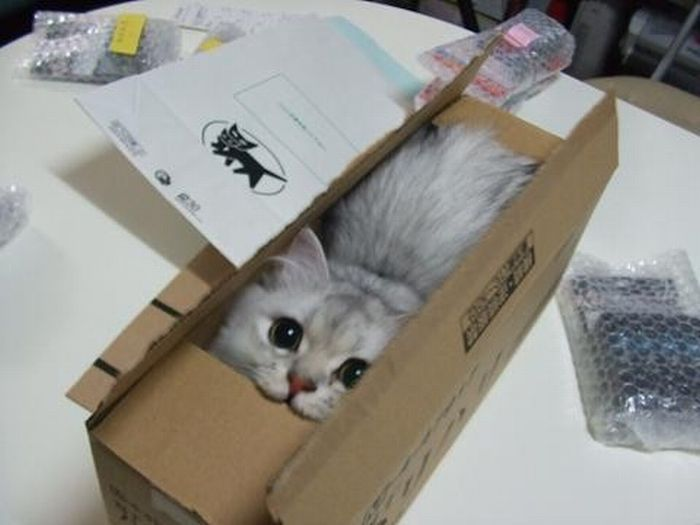
\includegraphics[width=\linewidth]{images/acatisfinetoo}
	\caption{\textit{Background modeling figure.}}
	\label{fig:BGModeling_fig} %Skapar referens till figuren
\end{figure}

\subsubsection{Solution}
A pixel that belongs to the background is static over time, as the background does not move. Each pixel is assigned a model for its variance over time, that is updated with each frame. With each frame, each pixel’s intensity is compared to the model and the deviation from the modeled intensity is the probability that the pixel belongs to an object not occluding the background.

Pixels determined to belong to the background in the previous frame will not have their probability models updated to prevent them from bleeding over into the background model.
This can be seen in figure \ref{fig:BGModeling_fig}. %Referens till figur, Ger klickbar länk i pdfen.


\newpage
\subsection{Foreground segmentation}
The Foreground segmentation is performed by the foreground processor module. The purpose of the foreground processor is to, from the probability map, decide which regions are interesting and create an object for each interesting region, and add these to the object vector of the frame. The shadow suppression is a part of the foreground processing. \\
\newline
The foreground processor is initiated by setting appropriate parameter values using the \emph{init} command. After being initiated, the foreground processor is called using the \emph{segmentForeground} command, which takes the current frame as an input. For more info, see appendix \ref{sec:ForeGroundSeg_code}.

\subsubsection{Morphological cleanup}
The first step in the foreground segmentation is to perform an initial simple cleanup of the background using one erode iteration. This performs a very good cleanup since most of the noise in the backround model is in form of single pixels, all of which are removed by the erode operation. After the first erode the shadow suppression algorithm is called to get rid of shadows, which the background model can't handle (see section 2.5). The output of the shadow suppression algorithm is then subject to several more steps of erode/dilate operations before the actual object detection.

%\begin{figure}[htb]
%	\centering
%	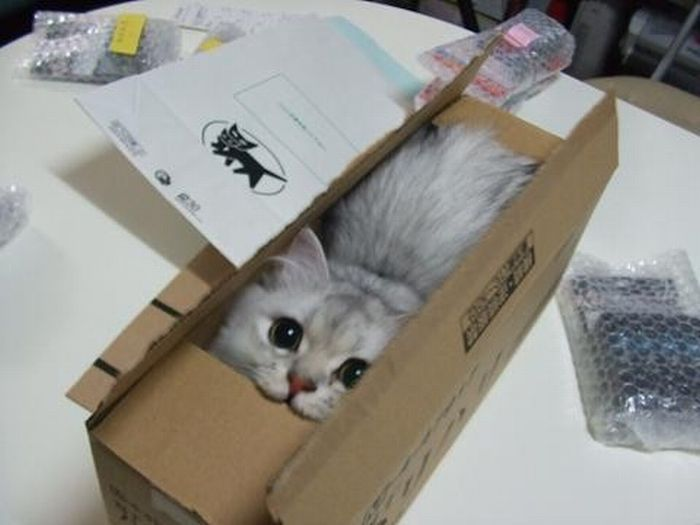
\includegraphics[width=\linewidth]{images/acatisfinetoo}
%	\caption{\textit{Some nice figure perhaps.}}
%	\label{fig:foreground_segmentation_fig} %Skapar referens till figuren
%\end{figure}

\subsubsection{Object detection}
To detect the regions the OpenCV command \emph{findContours} is used. For each detected contour, if it is large enough (to remove more garbage), a bounding rectangle of the type \emph{cv::Rect} is created and, from this rectangle an \emph{object} is created. All of the detected objects are then put into the Frame's object vector, and the foreground processing is complete.

\newpage
\subsection{Shadow suppression}
The shadow suppression is performed in a fashion similar to what is mentioned in the paper by Woods \cite{Wood}. The suppression if performed using the Hue- Saturation- Value- (HSV) mapping, The HSV mapping was chosen since it gives very small amounts of false positives and a manageable number of false negatives, while at the same time being fairly simple. We make the assumption that a if a pixel is shadowed the hue remains constant, while there is a decrease in both the value and saturation channels compared to the most likely background at the time.


\subsubsection{Implementation}
The Shadow Suppression function is called with a reference to \emph{frame} object containing both a processed version of the probability map, the current frame image as well as the most likely background. The first step is to remap the current frame image and the background model to the HSV-space. The suppression is performed by comparing all H- S- and V-values in the remapped images. If a pixel marked as foreground by the background model has a the same hue but lower saturation and value in the image than in the background model, it is assumed to be caused by a shadow, (eq. 3.19 in Wood \cite{Wood}). All probability map pixels assumed to be shadows are set to zero, and the shadow suppression is thereby finished.

\subsubsection{Parameters}
The parameters that need to be specified in the shadow suppression are the threshold values for the different channels, $\tau_H$, $\tau_S$, $\alpha$ and $\beta$. Let i denote the current image and m the currently most probable background. In order for a pixel to be classified as shadow, all of the following three constraints have to be fulfilled:

\begin{equation}
	|H_i - H_m| < \tau_H
	\label{eq:H}
\end{equation}
\begin{equation}
	S_i - S_m < \tau_S
	\label{eq:S}
\end{equation}
\begin{equation}
	\alpha_V < \frac{V_i}{V_m} < \beta_V
	\label{eq:V}
\end{equation}

The parameter setting depend on the scene that is being observed. For example in figure \ref{fig:shadow_suppression_fig} where most of the shadows are cast on a gray road (hue $\approx 0$), a rather large $\tau_H$ is required. Also, since the shadows are not so profound, alpha can be raised, causing lower false positives (non shadow pixels labeled as shadow pixels) for dark objects. There are big problems with false positives on dark objects in, for example, the Renova 0000 sequence. This is also seen to some extent in figure \ref{fig:shadow_suppression_fig}, from the Renova 0002 sequence.

\newpage
\begin{figure}[htb]
	\centering
	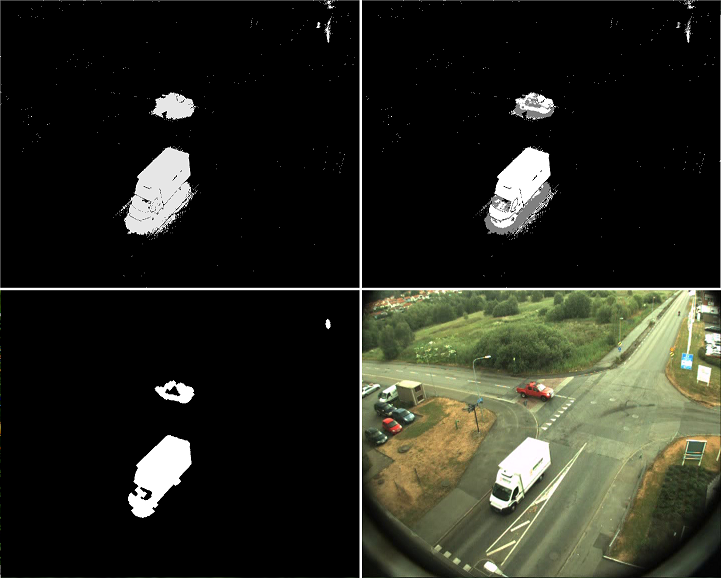
\includegraphics[width=\linewidth]{images/ShadowRenova0002.png}
	\caption{\textit{Renova image sequence 0002, frame 217. 
	\newline
	Top row: Background model output, model output with marked shadow pixels (gray) \newline
	Bottom row; final foreground image, actual video frame.}}
	\label{fig:shadow_suppression_fig}  %Skapar referens till figuren
\end{figure}

The parameters used to create the images in figure \ref{fig:shadow_suppression_fig} above were:

\begin{table}[htb]
\centering
\begin{tabular}{|c|c|}
	\hline
	Parameter & Value  \\
	\hline
	$\tau_H$ &  0.2 \\
	\hline
	$\tau_S$ & 0.5 \\
	\hline
	$\alpha$ &  0.5 \\
	\hline
	$\beta$ &  0.95 \\
	\hline
\end{tabular}

\caption{\textit{Parameters used to create figure \ref{fig:shadow_suppression_fig}.}}
\label{tab:shadow_parameters}
\end{table}

\newpage
\subsection{Object identification}
The purpose of \emph{Object identification} is to assign id's to objects discovered in the current frame based on what was known previous frames and using predictions from the Kalman filter. The aim is to assign a previously detected objects id to the most probable current object, or to none if the previous objects was moving out of the frame. New objects must be given new id's. Occlusion should be handled and objects that disappears by entering something or becoming stationary should be marked as lost but kept.

\subsubsection{Possible situations}
* Two objects move so close that they are estimated as one object by the foreground segmentation.
   - The new bounding box should approximately cover the two previous objects.
* ...

\subsubsection{Error measurement}
$$
  distanceError = (x_1 - x_2 - dx_2)^2 + (y_1 - y_2 - dy_2)^2
$$
$$
  areaError = (|width_1 - width_2| + |height_1 - height_2|)^2
$$
\\
$$
  Total error = distanceError + areaE
$$


\subsubsection{Algorithms}
See code in appendix \ref{sec:ObjID_code}. %referens till kod, ger klickbar länk.

\begin{figure}[htb]
	\centering
	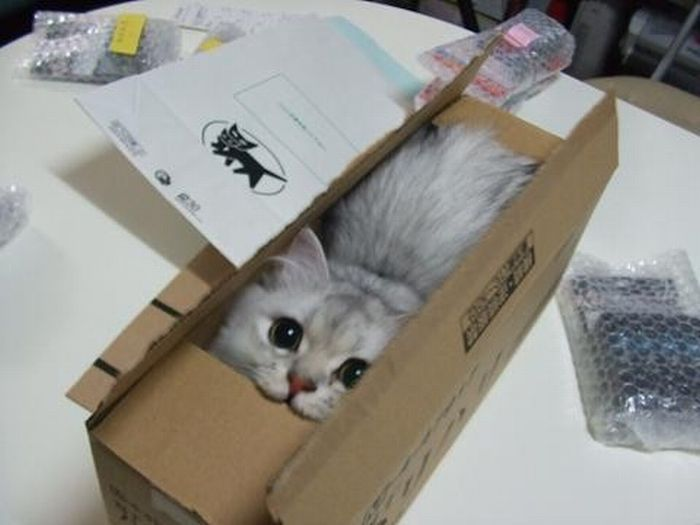
\includegraphics[width=\linewidth]{images/acatisfinetoo}
	\caption{\textit{Object Identification flowchart.}}
	\label{fig:ObjID_fig} %Skapar referens till figuren
\end{figure}


\newpage
\subsection{Kalman prediction}
When objects in the scene get occluded some how, it will be lost by the visual identification. This can happen for instance when two persons paths cross. Therefore a technique is needed to keep track of objects that is not observable at the moment. In this project a Kalman filter is used to predict the future path of objects. The prediction is also used to ease the matching process between frames. 

\subsubsection{Model}
The Kalman filter uses a state space model and a weighted average of the model prediction and new measurements to determine its estimate. The fundamental is seen in the equations below.


$$
\hat{\textbf{x}}_{k|k-1} = \textbf{A}\hat{\textbf{x}}_{k-1|k-1} +  \textbf{w}_{k-1}  
$$
$$
\hat{\textbf{y}}_{k|k} = \textbf{A}\hat{\textbf{x}}_{k|k} +  \textbf{v}_{k}
$$
	
$\hat{\textbf{x}}_{k|k-1}$ is an estimate the internal state vector at time $k$ given measurements at $k-1$. This is what we think we know about the object. The matrix A defines how the current state vector is used to estimate the next state vector. C defines the relation between measurements, $\hat{\textbf{y}}_{k|k}$, and the state vector. $\textbf{w}_{k}$ and $\textbf{v}_{k}$ are model- and measurement noise respectively. The Kalman filter also make use of $\textbf{Q}$ and $\textbf{R}$ which are the corresponding variance matrices to the noise sources. The last parameter needed is the covariance between the predicted state vector and the one that is measured. This is denoted $\textbf{P}_{k}$.

$$
\textbf{Q} = var(\textbf{w}_k), \forall k
$$
$$
\textbf{R} = var(\textbf{v}_k), \forall k
$$



\subsubsection{The Kalman Filter}
The Kalman filter is made up of two main parts; measurement update and time update. The measurement update takes as the name suggests a new measurement and updates the model according to this new measurement. The filter uses a matrix, $\textbf{K}$, referred to as the Kalman gain. This determines the mixture between old and new information.

\paragraph{Kalman Filter Algorithm}	

$$
\textbf{K}_{k} = \textbf{P}_{k-1}\textbf{C}^T(\textbf{C}\textbf{P}_{k-1}\textbf{C}^T + \textbf{R})^{-1}
$$
$$
\hat{\textbf{x}}_k = \hat{\textbf{x}}_{k-1} + \textbf{K}_k (\textbf{y}_k - \textbf{C}\hat{\textbf{x}}_{k-1})
$$
$$
\textbf{P}_k = \textbf{P}_{k-1} - \textbf{K}_k\textbf{C}\textbf{P}_{k-1}^T
$$

$$
\hat{\textbf{x}}_{k+1} = \textbf{A}\hat{\textbf{x}}_{k}
$$
$$
\textbf{P}_{k+1} = \textbf{A}\textbf{P}_{k}\textbf{A}^T + \textbf{Q}
$$

Depending on where the state vector is stored in the algorithm, either a filter or predictor is achieved. Since this project seeks a predictor the vector is stored in the time update.
 
See code in appendix \ref{sec:Kalman_code}. %referens till kod, ger klickbar länk.

\begin{figure}[htb]
	\centering
	%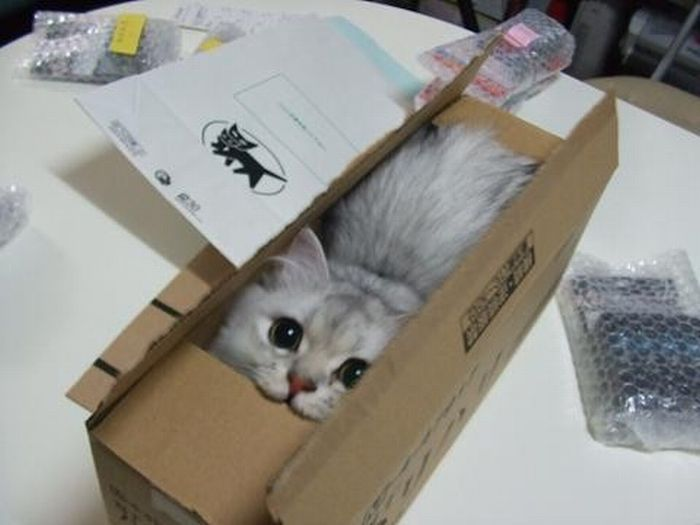
\includegraphics[width=\linewidth]{images/acatisfinetoo}
	\caption{\textit{Kalman Prediction figure.}}
	\label{fig:kalman_fig} %Skapar referens till figuren
\end{figure}

\newpage
\subsection{Occlusion handling}
\label{sec:Occlusion}
Occlusion should be handled and objects that disappears by entering something or by becoming stationary should be kept.

\subsubsection{Situations and solution strategies}
\begin{easylist}
& Two objects (or more) move so close that they are estimated as a single object by the foreground segmentation.
&& The new parent object should not be classified as an object, rather the previous objects should be kept.
&& The old objects should be updated according to their speed vector values of the occlusion moment using the predictor (no measurement update, only time update).
&& The objects should be within the border of the parent object.
&& The objects should only be as wide and high as the parent object, as a maximum restriction.

& An object is moving when it suddenly moves behind a hinder from the background and thus suddenly disappear, then it pop out on the other side of the hinder at a distance from its disappearance.
&& When the object disappear it is marked as lost and is updated according to its speed vector value of the moment of disappearance using the predictor (no measurement update, only time update) until the original object appears close to the estimation. The estimation and the 'new' object is considered the same object.

& An object move in the scene and suddenly stop.
&& The object is marked as lost and kept. When a newly discovered object is close enough it is considered to be the same object.
\end{easylist}


\newpage
\section{System Evaluation}
\label{sec:evaluation}
One of the most important parts of a project is the ability to evaluate it. Without it there is no way to compare results and grade your success. There exist no established evaluation method for multiple object tracking, but there are several candidates available. It was however decided to use two measures called MOTA, multiple object tracking accuracy, and MOTP, multiple object tracking precision. These are easy to grasp, implement and compare. The other group carrying out the same project uses the same measures which makes comparison between the groups easy.

\subsection{Ground Truth}
The evaluation needs access to some sort of ground truth which is defined as the best possible achievable tracking output. Through out this part of the document an object is defined as a position by the ground truth and a hypothesis as the output from the tracker. The method only allows one-to-one correspondence between objects and hypothesis and in case of conflict the combination yielding the lowest total distance error is chosen.

\subsection{MOTA}
MOTA is measure of accuracy with respect to how many mistakes are made by the tracker. It consists of four variables: misses, false positive, mismatches and number of objects. A miss is when no hypothesis is suggested close enough to an object. Close enough is defined by a threshold, T. This is the only design parameter in this method. If the distance between an object and the closest hypothesis is larger than T, the object yields a miss. If a hypothesis has no object within the threshold it results in a false positive error. One important feature of a tracker is the ability to keep objects identities correct. If this is not the case and an object is changing identity between frames one mismatch error is added for every change. The number of objects variable is defined as the total number of objects trackable according to the ground truth in the current frame. Finally to gain the MOTA calculate:
$$
1 - sum(misses +false positive+mismatches)/sum(number of objects)
$$

\subsection{MOTP}
The MOTP is a measure of how well the correct matches fit the ground truth objects. It only uses two variables: distance and matches. The distance is calculated between a hypothesis and its corresponding object. Matches is the number of hypothesis within the 
threshold, T, of an object. To gain MOTP calculate:

$$
sum(distance)/sum(matches)
$$



\begin{figure}[htb]
	\centering
%	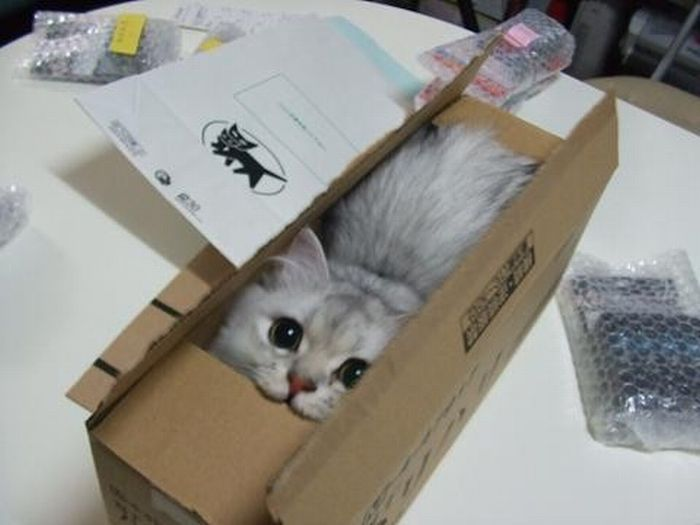
\includegraphics[width=\linewidth]{images/acatisfinetoo}
	\caption{\textit{System evaluation figure.}}
	\label{fig:system_evaluation_fig} %Skapar referens till figuren
\end{figure}





\newpage
\section{Results}
In this section the results of the project is summarized for some sequences chosen together with the other group. The sequences, as well as the ground truth used are provided by the EC Funded CAVIAR project, \cite{CAVIAR}.

\subsection{Evaluation Scores}

\begin{table}
\centering
	\begin{tabular}{r | c | c | c }
		\emph{Sequence Name}		& \emph{MOTA} & \emph{MOTP} \\
		\hline \hline
		OneLeaveShop1front			& 0.56 & 5.01 \\
		OneLeaveShop2front			& 0.70 & 5.30 \\
		OneLeaveShopReenter2front	& 0.65 & 5.09 \\
		OneStopNoEnter2front 		& 0.85 & 5.48 \\
		WalkByShop1front 			& -0.66 & 7.96 \\
	\end{tabular}
	\caption{\textit{Tracking performance according to the MOTA and MOTP evaluation standards, as described in section \ref{sec:evaluation}.}}
	\label{tab:evaluation_performance}
\end{table}

\subsection{Parameters}

\begin{table}
\centering
	\begin{tabular}{r | c || c | c || c | c | c | c | c }
	&	\multicolumn{1}{|c||}{BG model} & \multicolumn{2}{c||}{FG Segmentation} & \multicolumn{4}{c|}{Shadow Detection} \\
		\hline
		\emph{Sequence Name} & \emph{Learning Rate} & \emph{Iterations} & \emph{Min Thickness} &\emph{$\tau_H$} & \emph{$\tau_S$} & \emph{$\alpha$} & \emph{$\beta$}\\ 
		\hline \hline
		OneLeaveShop1front			& 0.05 		& 3 & 3.5 	& 0.5 & 1 & 0.8 & 0.99\\
		OneLeaveShop2front			& 0.05 		& 3 & 4 	& 0.5 & 1 & 0.8 & 0.99\\
		OneLeaveShopReenter2front	& 0.05		& 4 & 4 	& 0.5 & 1 & 0.8 & 0.99\\
		OneStopNoEnter2front 		& 0.033		& 3 & 4 	& 0.5 & 1 & 0.8 & 0.99\\
		WalkByShop1front 			& 0.033 	& 4 & 8 	& 0.5 & 1 & 0.8 & 0.99\\
	\end{tabular}
	\caption{\textit{Parameters used to receive the evaluation results presented in table \ref{tab:evaluation_performance}.}}
	\label{tab:evaluation_parameters}
\end{table}


\subsection{Performance}


\subsection{Technical Conclusion}
The evaluation needs access to some sort of ground truth which is defined as the best possible achievable tracking output. Through out this part of the document an object is defined as a position by the ground truth and a hypothesis as the output from the tracker. The method only allows one-to-one correspondence between objects and hypothesis and in case of conflict the combination yielding the lowest total distance error is chosen.

\subsection{Conclusion}
MOTA is measure of accuracy with respect to how many mistakes are made by the tracker. It consists of four variables: misses, false positive, mismatches and number of objects. A miss is when no hypothesis is suggested close enough to an object. Close enough is defined by a threshold, T. This is the only design parameter in this method. If the distance between an object and the closest hypothesis is larger than T, the object yields a miss. If a hypothesis has no object within the threshold it results in a false positive error. One important feature of a tracker is the ability to keep objects identities correct. If this is not the case and an object is changing identity between frames one mismatch error is added for every change. The number of objects variable is defined as the total number of objects trackable according to the ground truth in the current frame. For a sequence the equation for MOTA is found in \eqref{eq:MOTA}.






%
% Bibliography
%

% Force a blank page so the bibliography starts on a new page.
% Comment out if not necessary
\newpage
\thispagestyle{fancy}
\mbox{}
\newpage
\begin{thebibliography}{9}
\addcontentsline{toc}{section}{References} % Add an entry for this in the table of contents

\bibitem{CVBook}
	Sonka, M., Hlavac, V. \& Boyle, R. \\
	\emph{Image Processing, Analysis, and Machine Vision}.\\
	Toronto: Thompson Learning,\\
	cop. 2008, 3rd ed.,\\
	ISBN 0495244384.

\bibitem{levmar}
    Lourakis, M.I.A.\\
   \emph{levmar: Levenberg-Marquardt nonlinear least squares algorithms in {C}/{C}++}\\
     \verb+http://www.ics.forth.gr/~lourakis/levmar/+,\\
    Jul. 2004\\
    Accessed on May 14th 2005.
    
\bibitem{sparseLM}
    Manolis I.A. Lourakis\\
   ``Sparse Non-linear Least Squares Optimization for Geometric Vision,''\\
    \emph{European Conference on Computer Vision},\\
    vol.~2, 2010,
    pages~43-56 \\
    DOI \verb+http://dx.doi.org/10.1007/978-3-642-15552-9_4+

\bibitem{HZ}
	Hartley, R \& Zisserman, A\\
	\emph{Multiple View Geometry in Computer Vision}.\\
	Cambridge University Press, West Nyack, NY, USA \\
	March 2003, 2nd ed.\\
	ISBN 978--05--11--18711--7
	
\bibitem{Klas}
	Nordberg, K\\
	\emph{Introduction to Homogeneous Represenations and Estimation in Geometry}\\
	Apr. 2013\\
	Computer Vision Laboratory,	Department of Electrical Engineering\\
	Linköping University


	

%\bibitem{somePaper}
%	Q. Lastname,
%	``Some article title,''
%	\emph{Some scientific journal},
%	vol.~1337, no.~1337,
%	pp.~666--1337,
%	month.~1337.

\end{thebibliography}



%\begin{comment}

%
% Appendix start
%
\newpage
\appendix
\addcontentsline{toc}{section}{Appendices} % Add an entry for this in the table of contents

% Define background color for the code
\definecolor{sexy-gray}{gray}{0.95}

% Set properties for source code listings
\lstset{
	language=C++, 									% Language
	frame=single,									% Frame around code
	tabsize = 4,									% Better Tabbing
	basicstyle=\ttfamily\scriptsize,				% Font size and style
	commentstyle=\ttfamily\color{green!40!black},	% Comment color and style
	numbers=left,									% numbering
	backgroundcolor=\color{sexy-gray},				% background color
	keywordstyle=\color{blue},						% Keyword color
	stringstyle=\color{orange},						% String color
	showstringspaces=false,							% Don't show string spaces
	morekeywords={electrical, analog},  			% Additional keywords 
	breaklines = true, 								% Auto new line
	extendedchars = true,							% Allow more than ASCII chars
}


\section{Source code for data structures}
\subsection{Frame class}
\label{sec:Frame_code}
\lstinputlisting{../Modules/Frame.h}
\newpage
\lstinputlisting{../Modules/Frame.cpp}

\subsection{FrameList class}
\label{sec:FrameList_code}
\lstinputlisting{../Modules/FrameList.h}
\newpage
\lstinputlisting{../Modules/FrameList.cpp}

\subsection{Object class}
\label{sec:Object_code}
\lstinputlisting{../Modules/Object.h}
\newpage
\lstinputlisting{../Modules/Object.cpp}


\newpage
\section{Source code for Background modeling}
\label{sec:BGMod_code}
\subsection{Background Model}
\lstinputlisting{../Modules/BackgroundModelling/BackgroundModel.h}
%\newpage
\lstinputlisting{../Modules/BackgroundModelling/BackgroundModel.cpp}
\newpage
\subsection{Probability Map}
\label{sec:ProbMap_code}
\lstinputlisting{../Modules/BackgroundModelling/ProbabilityMap.h}
\newpage
\lstinputlisting{../Modules/BackgroundModelling/ProbabilityMap.cpp}

\newpage
\section{Source code for Foreground segmentation}
\label{sec:ForeGroundSeg_code}
\lstinputlisting{../Modules/ForegroundProcessing/ForegroundProcessor.h}
\newpage
\lstinputlisting{../Modules/ForegroundProcessing/ForegroundProcessor.cpp}

\newpage
\section{Source code for Object identification}
\label{sec:ObjID_code}
\lstinputlisting{../Modules/ObjectIdentification/Identification.h}
\newpage
\lstinputlisting{../Modules/ObjectIdentification/Identification.cpp}

\newpage
\section{Source code for Kalman prediction}
\label{sec:Kalman_code}
\lstinputlisting{../Modules/Prediction/Kalman.h}
\newpage
\lstinputlisting{../Modules/Prediction/Kalman.cpp}

\newpage
\section{Source code for Main program}
\label{sec:Main_code}
\lstinputlisting{../tracking.cpp}

% Set properties for Matlab code listings
\lstset{
	language=Matlab, 					% Language
	frame=single,						% Frame around code
	basicstyle=\small,					% Font size
	numbers=left,						% numbering
	backgroundcolor=\color{sexy-gray},	% background color
	morekeywords={textscan,ones},		% Additional keywords
}

%\lstinputlisting{code_files/Sigma_Delta_PSD_SNR_and_ENOB_calculations_INNAN_PILL.m}
%\end{comment}

\end{document}
